\documentclass{article} 
\usepackage{geometry}
\usepackage{cite}
\usepackage{amssymb}
\usepackage{float}
\usepackage[noend]{algpseudocode}
\usepackage{algorithmicx,algorithm}
\usepackage{graphicx}
\usepackage{subfigure}

\geometry{a4paper,left=2cm,right=2cm,top=1cm,bottom=1cm}
\title{Achieving the Highest Average User Data Rate in Wireless Network using Reinforcement Learning}
\author{Qi Cao, Mingqi Yuan, Simon Pun, Yi Chen, Siliang Zeng}
\date{\today}
\begin{document}
\maketitle
\section{Framework of Reinforcement Learning}
Reinforcement learning is learning what to do——how to map situations to actions——so as to maximize a numerical reward signal.
The learner is not told which actions to take, but instead must discover which actions yield the most reward by trying them 
\cite{Sutton1998Reinforcement}.Typically, an reinforcement learning system consists of two essential components:interaction 
environment and agent.With respect to RBG allocation, the scheduling process is discrete owing to its intrinsic motivation.
Thus the trajectory of interaction can be formulated as below: 
$$
S_0, A_0, R_1, S_1, A_1, R_2, S_2, A_2, R_3, ... ,S_{tti}, A_{tti}, R_{tti+1},...
$$
where $S \in \mathbb{S}$ is the state space, $A \in \mathbb{A}$ is the action space, $R \in \mathbb{R}$ is the reward space.
The following section describe the architecture of our reinforcement learning system in detail.
\subsection{Interaction environment}
The environment gives feedback to the actions made by the agent, including the status of the next state and rewards for the current actions.
For such a complex system as communication resource scheduling, the construction of state space is very challenging and valuable.
\paragraph{State}
In terms of RBG allocation, the state of environment is composed of status of all users in the base station.
That is to say, all the attributes are part of this state space, including the known and the unknown.
In order to establish an reasonable and quantitative state space, 
mutiple attributes were carefully seleteced from different layers of communication to characterize the state of interaction environment, 
and \textbf{Table 1} illustrates the details of those attributes.

\begin{table}[H]
    \centering
    \begin{tabular}{ccc}
    \hline
    Attr                    & Layer   & Dim       \\ \hline
    RSRP                    & physics & 1         \\
    Before scheduled buffer &         & 1         \\
    History avg rate        &         & 1         \\
    Olla offset             &         & 1         \\
    Scheduled times         &         & 1         \\
    RB CQI                  & physics & Num of RB \\
    $ \mu $(RB CQI)         & physics & 1         \\
    $ \sigma $(RB CQI)      & physics & 1         \\ \hline
    \end{tabular}
    \caption{Attributes of state}
\end{table}

Thus the dimension of state for each user is:
$$
dim_{state}=num_{RB}+7
$$
The construction of the subsequent deep neural network is also related to the specific dimension of the state.

\paragraph{Reward}
With regard to the learning system, the reward signal characterize the optimization target, which motivates the agent to explore any possible solutions.
The system aim to maximize the average rate of transmission, to this end, the configuration of reward function must take transmission rate into consideration.
The proposed reward function is formulated as below:

$$
r_{now} = \frac{r_{before}\cdot N\zeta + s}{N\zeta + \zeta} \quad N=tti_{now} - tti_{before} + 1
$$
$$
r_{\Delta }=r_{now}-r_{before}=\frac{s}{(N+1) \cdot \zeta}
$$
st.
$$ 
reward = \log_{\eta_{avg}}(\sum_{i=0}^{n}{r_{\Delta}}_{i}+1) 
$$

where $ r $ is transmission rate, $ s $ if effective tb size, $ \zeta $ is coeffcient.
In particular, the $\log$ function and $\eta_{avg}$ were introduced to ensure that the reward function is strictly incremental and locally bounded. 
A large number of experiments show that the boundedness of reward function will promote the convergence of the model during training.

\subsection{Agent}
The agent acts on observations of the environment, which is defined in \textbf{1.1}.
In the following section, the optimization algorithm and network design will be elaborated in detail, respectively.
\subsubsection{Deep Deterministic Policy Gradient}
The optimization algorithm gives the method of exploration and adjustment, a \textit{Deep Deterministic Policy Gradient} is introduced in this study,
which is model-free, off-policy actor-critic algorithm using deep function approximators that can learn policies in high-dimensional, continuous action spaces.
\cite{Lillicrap2015Continuous}
The actor network makes actions and the critic network estimates the reward,
so let $ \mu (s|\theta^{\mu}), s\in \mathcal{S} $ denote the actor and $ \mu (s|\theta^{Q}), s\in \mathcal{S} $ as critic, respectively.
To summarize, the application of DDPG for RBG allocation is illustrated in the \textbf{Algorithm 1}.

\begin{algorithm}
\caption{DDPG for RBG Allocation}
\begin{algorithmic}

\State Randomly initialize critic network $ Q(s, a|\theta^Q) $ and actor $ \mu (s|\theta^{\mu}) $ with weights $ \theta^Q $ and $ \theta^{\mu} $.
\State Initialize target network $ Q^\prime $ and $ \mu^\prime $ with weights $ \theta^{Q^\prime} \leftarrow \theta^Q $, $ \theta^{\mu^\prime} \leftarrow \theta^{\mu}$ 
\State Initialize replayer buffer $ B $, learning rate $ \tau $, Possion distribution $ P(X=k)=\frac{\lambda^k}{k!}e^{-k},k=0,1,...$
\For{Epoch=1, M}
\State Randomly initialize the user number $ K $ of current epoch
\State $ K $ users generated from environment
\State Receive initial observation state $ s_1 $ 
\For{tti=1, T}
\State Add users to base station according to Poisson distribution
\State Execute action $ a_{tti}=\beta(s_{tti}) $ and observe new state $ s_{tti+1} $
\State Receive reward $ r_{tti} $ and store the transitions $ (s_{tti}, a_{tti}, r_{tti}, s_{tti+1}) $ in $ R $
\State Sample a random minibatch of $ N $ transitions $ (s_i, a_i, r_i, s_{i+1}) $ from $ B $
\State Set $ y_i = r_i + \gamma Q^{\prime}(s_{i+1}, \mu^{\prime}(s_{i+1}|\theta^{\mu^{\prime}})|\theta^{Q^{\prime}}) $
\State Update critic by minimizing the loss:$ L=\frac{1}{N} \sum_{i}(y_i - Q(s_i, a_i|\theta_Q)^2)$
\State Update the actor policy using the sampled gradient:
$$
\nabla_{\theta^{\mu}}\mu|_{s_i}\approx \frac{1}{N}\sum_i \nabla_{a}Q(s, a|\theta^Q)|_{s=s_i,a=\mu(s_i)}\nabla_{\theta^{\mu}}\mu(s|\theta^{\mu})|_{s_i}
$$
\State Update the target networks:
$$
\theta^{Q \prime} \leftarrow \tau\theta^{Q} + (1-\tau)\theta^{Q \prime}
$$
$$
\theta^{\mu \prime} \leftarrow \tau\theta^{\mu} + (1-\tau)\theta^{\mu \prime}
$$
\EndFor
\EndFor
\end{algorithmic}
\end{algorithm}


This RBG allocation task belongs to discrete action space, however, the DDPG is designed for continuous action space.
To make the discrete task become continuous will contibute to the model convergence. 
In the early stage of proof, algorithms based on stochastic policy, such as Soft-AC \cite{HaarnojaSoft}, 
had also been tried, but the model often fail to converge.

\subsubsection{RBGNet}
In the real communication process, the number of users in the base station changes frequently, 
it means that the state submitted to the agent is not always the same dimension, which leads to great challenges to the network design of the actor and critic.
Traditional full connected neural network is widely used in deep Q-learning, but it's limited by its fixed input and output.
To address this problem, convolutional neural network is adopted to build the two components, 
which can accept scalable input when the network is fully convolutional. \cite{long2015fully}
This network structure designed for RBG Allocation is named \textbf{RBGNet}

\paragraph{Backbone}
\textbf{Figure 1} illustrates the architecture of RBGNet.
\begin{figure}[h]
\centering
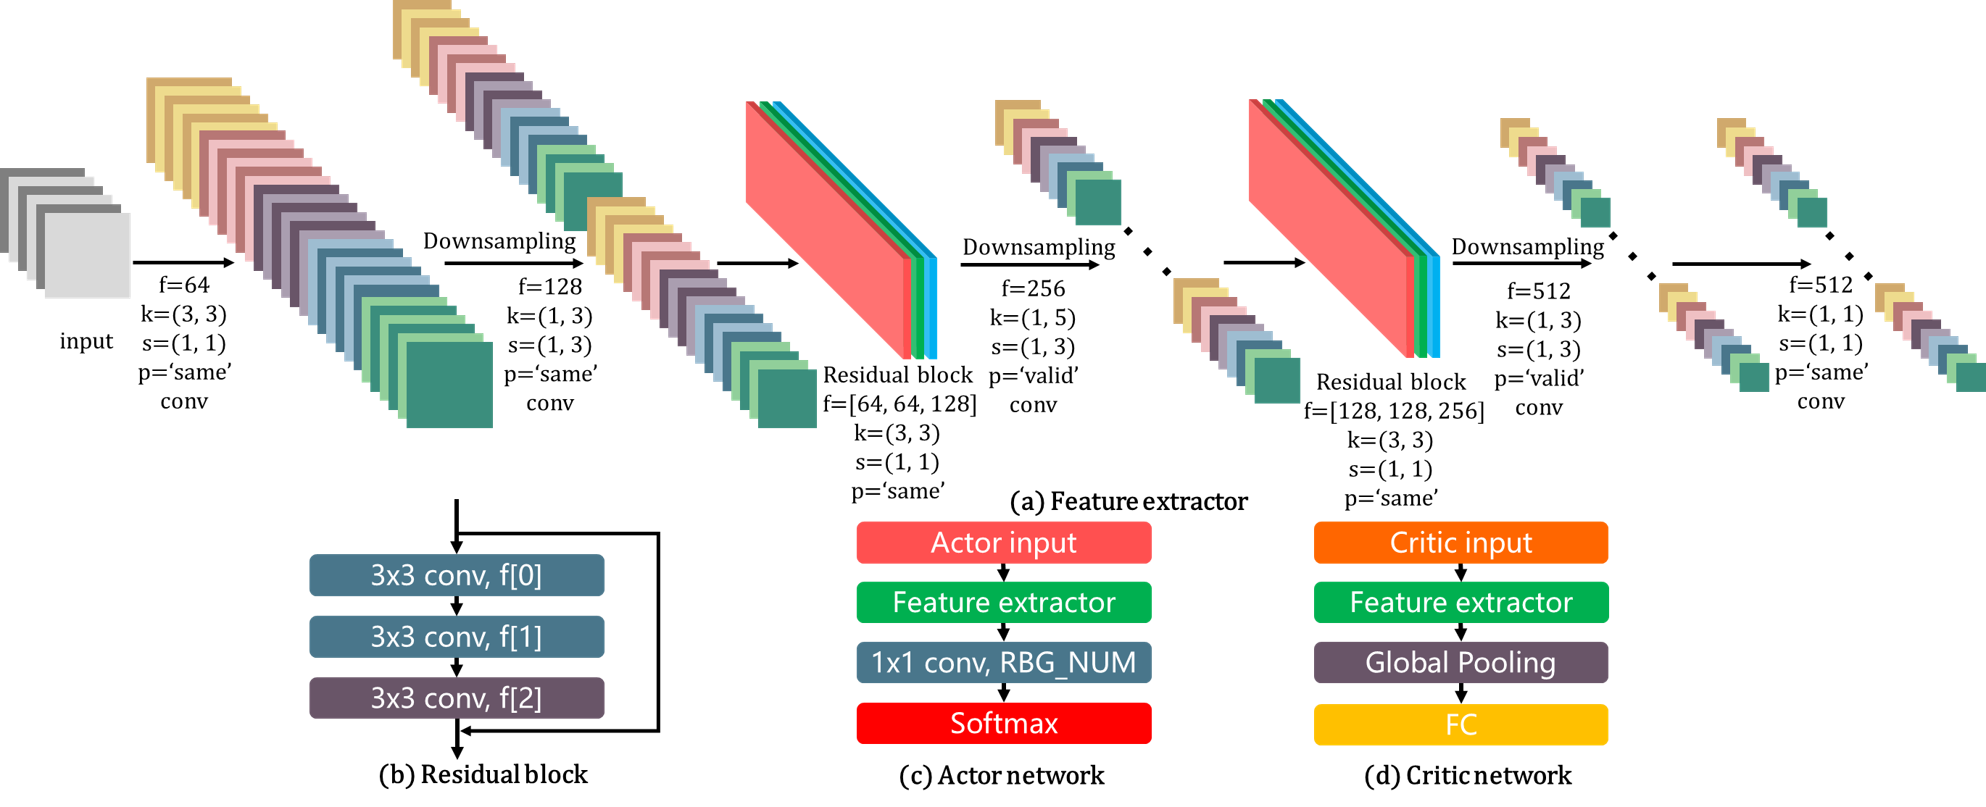
\includegraphics[width=16cm]{RBGNet}
\caption{Architecture of RBGNet.The parameters of downsampling layers were configured skillfully based on $ dim_{feature} $ }.
\end{figure}
The actor and critic take the same feature extractor to handle the input, 
which can effectively simplify the design of architecture and adjustment of network parameters.
It's worth mentioning that the network is so deep that two residual block is inserted to avoid the gradient disappearing. \cite{He2016Deep}
Also, the very deep network obtains more powerful learning ability to address such a complex problem. 

\paragraph{Remark}
For the actor network, the input's shape is: 
$$ 
dim_{actor \, input}=(batch \, size, dim_{state}, K, 1)
$$
where $ K $ is the quantity of user, $ 1 $ is regarded as channel of image processing.
Apply downsampling to the input for three times, the shape of output map is: 
$$
dim_{output \, map}=(batch \, size, K, 1, F) 
$$
where $ F $ is the quantity of filters in the last convolution layer of feature extractor.
As shown above, the third dimension of $ dim_{output \, map} $ is $ 1 $, which is necessary for the subsequent process, 
so the parameters of downsampling layer should be configured skillfully based on the $ dim_{state} $.

Then, this map is submitted to the output layer, which is a convolution layer with (1, 1) filters and Softmax activation function, and 
the Softmax score characterizes the allocation result.
Specially, the quantity of filters in the output layer is equal to the quantity of RBG, which aims to make each RGB be allocated by
an independent filter.
Based on the configuration, each RBG was allocated independently but the prediction is still joint.
The final result has nothing to do with the $ dim_{state} $ but only related to the quantity of users and RBG.
$$
dim_{softmax \, score}=(batch \, size, K, 1, Num_{RBG})
$$

For the critic network, the input is the integration of state and action, thus the input's shape is 
$$ 
dim_{critic \, input}=(batch \, size, dim_{state}+Num_{RBG}, K, 1) 
$$
Firstly, the input is submitted to feature extractor to produce intermediate feature.
Secondly this map is processed by the Global Pooling layer, which can replace the fully connected layer to accept scalable input. \cite{Lin2013Network}
Thus the output is only related to the quantity of filters in the last convolution layer of feature extractor.
$$
dim_{output \, map}=(batch \, size, F) 
$$
Finally, this map is received by a fully connected layer to predict the reward.

\subsubsection{Training strategy}
The training of reinforcement learning is a difficult and long-time job.
In the early stage of the experiment, two models were established to solve the problem of full buffer case and bursty case respectively.

\begin{algorithm}
\caption{Training strategy}
\begin{algorithmic}
\State \textbf{Step 1: full buffer case training}
\State
Initialize agent $\mathcal{A}_{RL}$ and $\mathcal{A}_{Oppo}$ respectively.
\State  
Initialize $p(\mathcal{A}_{RL}) \leftarrow 0, p(\mathcal{A}_{Oppo}) \leftarrow 0$, where $ p() $ is the performance of agent, threshold $ \varphi_{1} $.
\While{$ p(\mathcal{A}_{Oppo}) - p(\mathcal{A}_{RL}) > \varphi_{1} $}
    \For{Epoch=1, M}
    \State Two agents interact with the environment to generate available experience $ E_{RL}^1$ and $E_{Oppo}^1$.
    \State Update $ \mathcal{A}_{RL} $ with \textbf{Mixed Experience} composed of $ E_{RL}^1$ and $E_{Oppo}^1$.
    \EndFor
    \State Update $p(\mathcal{A}^{\prime}_{RL})$ and $p(\mathcal{A}^{\prime}_{Oppo})$:
    $
    p(\mathcal{A}_{RL}) \leftarrow p(\mathcal{A}^{\prime}_{RL}), p(\mathcal{A}_{Oppo}) \leftarrow p(\mathcal{A}^{\prime}_{Oppo})
    $
    \If{$p(\mathcal{A}^{\prime}_{RL}) > p(\mathcal{A}_{RL})$}
    \State Update $\mathcal{A}_{RL}$: $ \mathcal{A}_{RL} \leftarrow \mathcal{A}^{\prime}_{RL} $
    \Else
    \State continue
    \EndIf
\EndWhile
\State Save the best agent model $ \mathcal{A}^{*}_{RL} $
\State \textbf{Step 2: bursty case training}
\State
Initialize agent:$\mathcal{A}_{RL} \leftarrow \mathcal{A}^{*}_{RL}$
\State
Initialize $p(\mathcal{A}_{RL}) \leftarrow 0, p(\mathcal{A}_{Oppo}) \leftarrow 0$, threshold $ \varphi_{2} $
\While{$ p(\mathcal{A}_{RL}) - p(\mathcal{A}_{Oppo}) < \varphi_{2} $}
\For{Epoch=1, M}
\State Two agents interact with the environment to generate available experience $ E_{RL}^2$ and $E_{Oppo}^2$.
\State Update $ \mathcal{A}_{RL} $ with $ E_{RL}^2$.
\State Update $p(\mathcal{A}^{\prime}_{RL})$ and $p(\mathcal{A}^{\prime}_{Oppo})$:
    $
    p(\mathcal{A}_{RL}) \leftarrow p(\mathcal{A}^{\prime}_{RL}), p(\mathcal{A}_{Oppo}) \leftarrow p(\mathcal{A}^{\prime}_{Oppo})
    $
\EndFor
\If{$p(\mathcal{A}^{\prime}_{RL}) > p(\mathcal{A}_{RL})$}
\State Update $\mathcal{A}_{RL}$: $ \mathcal{A}_{RL} \leftarrow \mathcal{A}^{\prime}_{RL} $
\Else
\State continue
\EndIf
\EndWhile
\end{algorithmic}
\end{algorithm}

For bursty case, the agent can explore any possible solutions to maximize the average transmission rate since the optimal solutions is uncertain, 
and the performance of the agent successfully surpasses the \textit{Opportunistic Schedule} after lots of training.

For full buffer case, the agent was hoped to achieve the effect close to that method, 
but we've found it's difficult to achieve that only by the agent's own exploration.
\textit{Opportunistic Schedule} is a fixed method, 
so it's difficult and impractical for a network with millions of parameters to learn a fixed method by trial-and-error.
Howerver, it's clear that the \textit{Opportunistic Schedule} is the optimal solution to maximize average rate, 
which provides the best experience to guide the agent.
Therefore, the \textbf{Mixed Experience} was introduced to train the agent, which is composed of the experience both from self-exploration and \textit{Opportunistic Schedule}.
With lots of training and \textit{fine-tuning} \cite{HowardUniversal}, the agent successfully simulated the \textit{Opportunistic Schedule}.

In order to make the model compatible with both full buffer case and bursty case, a step-by-step training strategy was introduced to address this problem.
First of all, the agent is trained with \textbf{Mixed Experience} in full buffer case, which can simulate the behavior of \textit{Opportunistic Schedule}.
At this stage, the \textit{fine-tuning} operation should be repeated again and again to get the best performance.

Secondly, using bursty case to train the previous model with low learning rate.Now, the experience is not mixed, which is only from the self-exploration.
In a word, the training strategy is full of technique which should be configuration based on the specific situation.

\bibliography{ref}
\bibliographystyle{ieeetr}
\end{document}

